\documentclass[12pt]{article}
\usepackage{titling}
\usepackage[absolute]{textpos}
\setlength{\TPHorizModule}{10mm}
\setlength{\TPVertModule}{10mm}
\usepackage[top=2.5cm, bottom=2.5cm, left=3cm, right=2.5cm]{geometry}
\usepackage[polish]{babel}
\usepackage{polski}
\usepackage[utf8]{inputenc}
\usepackage{graphicx}
\usepackage{floatrow}
\usepackage{listings}
\usepackage{color}
\linespread{1.5}
\title{Narzędzie wspomagające tworzenie ciągów przetwarzania wideo w oparciu o bibliotekę GStreamer}
\author{Marcin Kolny}
\usepackage[T1]{fontenc}
\usepackage{helvet}
\renewcommand*{\familydefault}{\sfdefault}
\renewcommand{\maketitle}{
  \begin{titlepage}
    \begin{figure}  
      
\includegraphics[width=40mm]{img/polsl-logo.png}
    \end{figure}
    \begin{center}
      \begingroup
      \fontsize{18pt}{21pt}\selectfont
      \textbf{Politechnika Śląska\\
        Wydział Automatyki, Elektroniki i Informatyki\\
        Kierunek Informatyka}\\
      \vspace{22mm}
      Projekt inżynierski\\
      \vspace{22mm}
      \endgroup
      \begingroup
      \fontsize{14pt}{17pt}\selectfont
      \thetitle \\
      \endgroup
      \vspace{30mm}
    \end{center}
    \begin{textblock}{14}(2.5,21.5)
      \fontsize{14pt}{17pt}\selectfont
      Autor: \theauthor \\
      Kierujący pracą: dr Ewa Lach\\
    \end{textblock}
    \begin{textblock}{20}(2.5,26.5)
      \fontsize{14pt}{17pt}\selectfont
      Gliwice, styczeń 2014\\
    \end{textblock}

  \end{titlepage}
}
\begin{document}
\definecolor{cppred}{rgb}{0.6,0,0} % strings
\definecolor{cppgreen}{rgb}{0.25,0.5,0.35} % comments
\definecolor{cpppurple}{rgb}{0.5,0,0.35} % keywords
\definecolor{cppblue}{rgb}{0.25,0.35,0.75} % doxygen
\definecolor{lightgrey}{rgb}{0.9,0.9,0.9}
\lstset{language=C++,
basicstyle=\ttfamily,
keywordstyle=\color{cpppurple}\bfseries,
stringstyle=\color{cppred},
commentstyle=\color{cppgreen},
morecomment=[s][\color{cppblue}]{/**}{*/},
numbers=left,
backgroundcolor=\color{lightgrey},
numberstyle=\tiny\color{black},
stepnumber=1,
numbersep=10pt,
tabsize=4,
showspaces=false,
showstringspaces=false}
\maketitle
\tableofcontents
\cleardoublepage
\section{Analiza problemu}
\subsection{Narzędzia}
\subsubsection{Biblioteka GStreamer}
\paragraph{}
Biblioteka GStreamer służy do konstruowania grafów przetwarzania strumieni multimedialnych. Biblioteka została napisana w języku ANSI C i dostępna jest pod systemami Linux, Windows, OS X oraz Android.

GStreamer wydany jest na licencji GNU GPL i może być wykorzystywany w zastosowaniach komercyjnych. Licencja pozwala również na modyfikowanie i dystrybucję kodu źródłowego biblioteki.
Biblioteka oferuje użytkownikowi wiele gotowych elementów do przetwarzania wideo (np. enkodery czy dekodery audio-video), do generowania sygnałów multimedialnych, a także do prezentacji wyników użytkownikowi. Ponadto, istnieje możliwość pisania własnych elementów, które można następnie użyć w bilbliotece GStreamer.

Biblioteka GStreamer oparta jest o \textbf{elementy} (ang. \textit{elements}). Elementem nazywany jest obiekt, który realizuje zadany algorytm. Przykładowym elementem jest dekoder, którego celem jest dekodowanie strumienia multimedialnego o zadanym formacie.

Element może zawierać gniazda, dzięki którym możliwe jest połączenie go z innymi elementami.

Elementy dzielą się na te, które zawierają tylko gniazda wejściowe (ang. \textit{sink elements}), które posiadają tylko gniazda wejściowe (ang. \textit{source elements}), oraz elementy zawierające zarówno gniazda wejściowe, jak i wyjściowe (ang. \textit{filter elements}).
\begin{figure}[H]
  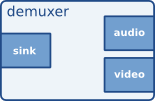
\includegraphics[width=40mm]{img/sample-demuxer.png}
  \caption{Przykładowy element typu \textit{demuxer} \cite{gstmainpage}}
  \label{fig:sampleDemuxer}
\end{figure}
\paragraph{}
Rysunek ~\ref{fig:sampleDemuxer} przedstawia przykładowy element, zawierający dwa gniazda wyjściowe, i jedno gniazdo wejściowe (jest to szczególny wariant filtra, tzw. \textit{demuxer}).
\paragraph{}
\textbf{Kontener} (ang. \textit{bin}) jest szczególnym elementem. Podobnie, jak elementy, kontenery posiadają gniazda. Natomiast algorytmy zdefiniowane w elemencie-kontenerze realizowane są poprzez inne elementy, które agregowane są w danym kontenerze. Rysunek ~\ref{fig:sampleBin} przedstawia przykładowy kontener, zawierający dwa elementy, oraz jedno gniazdo wejściowe.
\begin{figure}[H]
  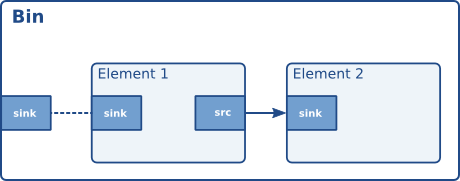
\includegraphics[width=100mm]{img/sample-bin.png}
  \caption{Przykładowy kontener \cite{gstmainpage}}
  \label{fig:sampleBin}
\end{figure}
\paragraph{}
\textbf{Strumień} (ang. \textit{pipeline}) jest specjalnym przypadkiem kontenera. Jest to kontener nadrzędny całego modelu programu. Przechowuje w sobie główne elementy oraz kontenery agregujące inne obiekty przetwarzające. Strumień nie posiada żadnych gniazd. Rysunek ~\ref{fig:samplePipeline} przedstawia przykładowy strumień, realizujący operację odtwarzania strumienia audio-video z pliku ogg.
\begin{figure}[H]
  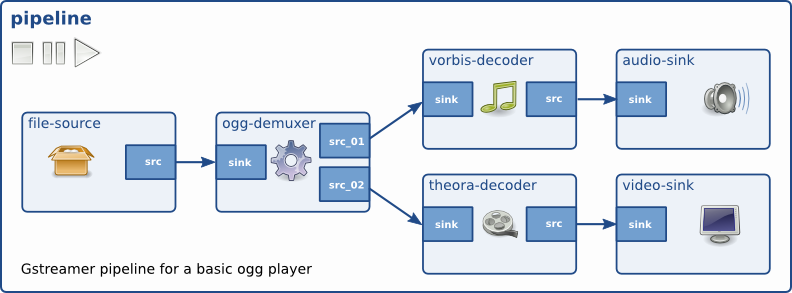
\includegraphics[width=150mm]{img/simple-player.png}
  \caption{Przykładowy strumień \cite{gstmainpage}}
  \label{fig:samplePipeline}
\end{figure}
\paragraph{}
\textbf{Gniazda} (ang. \textit{pads}) to obiekty umożliwiające połączenie ze sobą dwóch różnych elementów. Gniazdo charakteryzuje się dwoma właściwościami: kierunkiem oraz dostępnością. Pod względem kierunku, gniazda podzielone są na dwie grupy:
\begin{itemize}
 \setlength{\itemsep}{0em}
  \item wejściowe (ang. \textit{sink pads}),
  \item wyjściowe (ang. \textit{src pads}).
\end{itemize}

Gniazda wyjściowe (źródłowe), służą do przesyłania danych do następnego elementu. Gniazda wejściowe wykorzystywane są natomiast do odbierania danych przesłanych z poprzednich elementów.

Kolejna właściwość, dzieli zbiór gniazd na trzy grupy:
\begin{itemize}
 \setlength{\itemsep}{0em}
  \item występujące zawsze (ang. \textit{always pads}),
  \item występujące w zależności od danych (ang. \textit{sometimes pads, dynamic pads}),
  \item pojawiające się na żądanie użytkownika (ang. \textit{request pads}).
\end{itemize}

Gniazda należące do pierwszej grupy występują zawsze w elemencie, i nie można ich usunąć.
Druga grupa gniazd, to takie, które pojawiają się tylko wtedy, kiedy wystąpi taka potrzeba. Na rysunku ~\ref{fig:requestPadsDemux} pokazane zostały dwa demultiplexery połączone z elementem wczytującym dane z pliku. W pierwszym przypadku (po lewej), w pliku zapisane zostały dwa strumienie multimedialne, dla tego element \textit{ogg-demuxer} zawiera dwa gniazda źródłowe. W drugim przypadku (po lewej), plik zawiera tylko jeden strumień multimedialny, stąd demuxer wygenerował tylko jedno gniazdo.
\begin{figure}[H]
  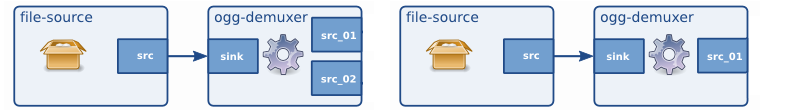
\includegraphics[width=150mm]{img/request-pads-demux.png}
  \caption{Dynamiczne gniazda elementu demuxera \cite{gstmainpage}}
  \label{fig:requestPadsDemux}
\end{figure}
Ostatnia grupa, to gniazda, pojawiające się na żądanie użytkownika. Można wyobrazić sobie odwrotną sytuację do opisywanej w poprzednim akapicie. Użytkownik wstawia element typu \textit{muxer}, który łączy kilka strumieni. W zależności od tego, ile strumieni użytkownik będzie chciał połączyć, tyle żądań o gniazdo wejściowe będzie musiał zgłosić.

\textbf{Połączenia} (ang. \textit{links}) pomiędzy dwoma elementami odbywają się przez tzw. \textit{negocjacje}. Każde gniazdo elementu posiada właściwość określającą, jakiego typu dane akceptuje dane gniazdo. Właściwości te nazywane są możliwościami (ang. \textit{capabilities}, \textit{caps}). Proces negocjacji ma na celu odnalezienie wspólnego formatu danych, jaki może zostać zaakceptowany przez odybwa gniazda (gniazdo wejściowe oraz wyjściowe), które użytkownik chce ze sobą połączyć. Jeśli negocjacje zakończą się niepowodzeniem (to znaczy, nie uda się znaleźć wspólnego formatu), połączenie nie zostanie wykonane.

\subsubsection{Adapter C++ - gstreamermm}
\paragraph{}
Adapter (ang. \textit{wrapper}) jest wzorcem projektowym, który ma na celu współdzielenie interfejsu pomiędzy dwoma blokami kodu źródłowego. Biblioteka GStreamer została napisana w języku ANSI C, dla tego, aby umożliwić programistom innych języków korzystanie z biblioteki, nie mieszając różnych języków, powstało kilka adapterów dla innych języków programowania (np. C++ czy C\#).

Biblioteka \textbf{gstreamermm} to projekt, którego celem jest stworzenie biblioteki-adaptera w języku C++ dla biblioteki GStreamer. Projekt rozwijany jest na licencji LGPL, dla tego każdy może uzyskać dostęp do kodu źródłowego biblioteki, a także w dowolny sposób modyfikować źródła.

Biblioteka gstreamermm należy do rodziny projektów pochodzących od projektu biblioteki-wrappera \textbf{gtkmm}. Biblioteka gtkmm umożliwia użytkownikowi korzystanie z funkcjonalności biblioteki GTK+, posługując się interfejsem napisanym w języku C++. Projekty oparte o fragmenty kodu biblioteki gtkmm, opierają się głównie o generowanie kodu źródłowego w języku C++ na podstawie źródeł napisanych w języku ANSI C. Wszystkie projekty korzystają ze wspólnych generatorów kodu, dla tego każde usprawnienie generatora w jednym projekcie, powoduje polepszenie jakości kodu w pozostałych projektach..

Kod źródłowy biblioteki jest w większości generowany automatycznie na podstawie źródeł projektu GStreamer w trójetapowym procesie. Rysunek ~\ref{fig:mmGenerateProcess} prezentuje wszystkie trzy kroki procesu generacji kodu źródłowego.
\begin{figure}[H]
  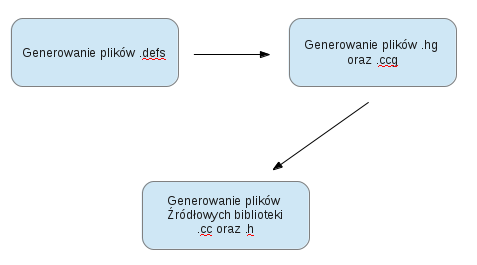
\includegraphics[width=100mm]{img/mm-generate-process.png}
  \caption{Schemat procesu generacji kodu źródłowego biblioteki gstreamermm}
  \label{fig:mmGenerateProcess}
\end{figure}
Pierwszym etapem generacji kodu jest przeszukanie źródeł biblioteki GStreamer, a następnie wygenerowanie plików definicji. Pliki definicji zawierają informacje na temat typów wyliczeniowych zdefiniowanych w bibliotece, funkcji, sygnałów, metod wirtualnych czy struktur danych. W przypadku wygenerowania przez generator błędnej definicji, stosowane są pisane przez programistę tzw. \textit{łatki} (ang. \textit{patch}).

W kolejnym przebiegu, generator na podstawie plików definicji, generuje pliki \textit{.hg} oraz \textit{.ccg}. Zawartość plików przypomina składnią język C++, jednak zawiera wywołania makrodefinicji ułatwiających adaptowanie poszczególnych elementów biblioteki. Przykład użycia makrodefinicji przedstawiony został na listingu ~\ref{macroSampleUsage}.
Listę dostępnych makr można znaleźć w dokumentacji projektu gnome \cite{devgnomepage}.
    \begin{lstlisting}[caption=Przykład użycia makrodefinicji w pliku \textit{.hg}, label=macroSampleUsage]
_WRAP_METHOD(bool load_preset(const Glib::ustring& name), 
      gst_preset_load_preset)
    \end{lstlisting}
    W przypadku, gdy plik \textit{.hg} zostanie niepoprawnie wygenerowany, programista zmuszony jest do ręcznego napisania tego pliku. W tym wypadku nie stosuje się łatek, ponieważ w większości przypadków, błąd obejmuje większą część pliku, a nie pojedyncze linie.

Ostatni etap generacji kodu źródłowego, to przekształcenie plików \textit{.hg} oraz \textit{.ccg} w pliki źródłowe języka C++. Na przykład, line pokazane na listingu ~\ref{macroSampleUsage} zostanie zastąpione kodem zaprezentowanym na listingu ~\ref{outMacroSampleUsage}.
    \begin{lstlisting}[caption=Kod źródłowy wygenerowany na podstawie makrodefinicji, label=outMacroSampleUsage]
bool load_preset(const Glib::ustring& name);
...
bool Preset::load_preset(const Glib::ustring& name)
{
  return gst_preset_load_preset(gobj(), name.c_str());
}
    \end{lstlisting}
    Funkcja \textit{gst\_preset\_load\_preset} jako drugi argument, przyjmuje wartość typu \textit{gchar*}. Generator wiedział, w jaki sposób dokonać konwersji na ten typ z typu \textit{const Glib::ustring\&}. Baza wiedzy, dotycząca konwersji pomiędzy typami ANSI C a typami języka C++, znajduje się w osobnych plikach, pisanych przez programistę.
W tym etapie, wygenerowany kod źródłowy jest zawsze poprawny. Programista może jedynie dopisać dodatkowe pliki. Przechowują one na ogół klasy usprawniające (ale nie rozszerzające funkcjonalność) pracę z biblioteką.
\cleardoublepage
\section{Specyfikacja zewnętrzna}
\subsection{Proces instalacji biblioteki gstreamermm}
Na listingu ~\ref{gstreamermmInstall} przedstawiony został zestaw poleceń, jakie należy wykonać w celu instalacji biblioteki gstreamermm. Proces instalacji wymaga połączenia z internetem, ponieważ źródła biblioteki muszą zostać pobrane ze zdalnego repozytorium.
\begin{lstlisting}[caption=Polecenia kompilujące program gst-creator, label=gstreamermmInstall]
[m.kolny@m.kolny-cmp ~]$ git clone git://
                             git.gnome.org/gstreamermm
[m.kolny@m.kolny-cmp ~]$ cd gstreamermm
[m.kolny@m.kolny-cmp gstreamermm]$ 
[m.kolny@m.kolny-cmp gstreamermm]$ ./autogen.sh
[m.kolny@m.kolny-cmp gstreamermm]$ make
[m.kolny@m.kolny-cmp gstreamermm]$ sudo make install
\end{lstlisting}

\subsubsection{Wymagane zależności dla kompilacji biblioteki}
Poniżej znajduje się lista zależności, jakie muszą zostać spełnione w celu poprawnej kompilacji i instalacji biblioteki gstreamermm:
\begin{itemize}
  \setlength{\itemsep}{0em}
\item narzędzie mm-common w wersji 0.9.6 lub wyższej,
\item biblioteka giomm-2.4 w wersji 2.36.0 lub wyższej,
\item biblioteka gstreamer-1.0 w wersji 1.0.10 lub wyższej,
\item biblioteka gstreamer-app-1.0 w wersji 1.0.10 lub wyższej,
\item biblioteka gstreamer-audio-1.0 w wersji 1.0.10 lub wyższej,
\item biblioteka gstreamer-base-1.0 w wersji 1.0.10 lub wyższej,
\item biblioteka gstreamer-check-1.0 w wersji 1.0.10 lub wyższej,
\item biblioteka gstreamer-controller-1.0 w wersji 1.0.10 lub wyższej,
\item biblioteka gstreamer-fft-1.0 w wersji 1.0.10 lub wyższej,
\item biblioteka gstreamer-net-1.0 w wersji 1.0.10 lub wyższej,
\item biblioteka gstreamer-pbutils-1.0 w wersji 1.0.10 lub wyższej,
\item biblioteka gstreamer-plugins-base-1.0 w wersji 1.0.10 lub wyższej,
\item biblioteka gstreamer-riff-1.0 w wersji 1.0.10 lub wyższej,
\item biblioteka gstreamer-rtp-1.0 w wersji 1.0.10 lub wyższej,
\item biblioteka gstreamer-sdp-1.0 w wersji 1.0.10 lub wyższej,
\item biblioteka gstreamer-tag-1.0 w wersji 1.0.10 lub wyższej,
\item biblioteka gstreamer-video-1.0 w wersji 1.0.10 lub wyższej.
\end{itemize}
Ponadto, w celu kompilacji przykładowych programów wykorzystujących bibliotekę gstreamermm, w systemie musi być zainstalowana biblioteka gtkmm-3.0 w wersji 3.0 lub wyższej.
\subsection{Proces instalacji programu}
Oprogramowanie dostarczane jest w postaci kodu źródłowego, dla tego w celu uruchomienia programu, należy dokonać kompilacji programu. Skrypt budujący został przygotowany pod narzędzie \textbf{CMake}. Aby skompilować program, należy wykonać polecenia w konsoli przedstawione na listingu ~\ref{compileProject} (użytkownik powinien znajdować się w katalogu głównym repozytorium programu).
\begin{lstlisting}[caption=Polecenia kompilujące program gst-creator, label=compileProject]
[m.kolny@m.kolny-cmp gst-creator]$ mkdir build
[m.kolny@m.kolny-cmp gst-creator]$ cd build/
[m.kolny@m.kolny-cmp build]$ cmake ..
[m.kolny@m.kolny-cmp build]$ make
[m.kolny@m.kolny-cmp build]$ ./src/gst-creator &$
\end{lstlisting}
Polecenia spowodują skompilowanie aplikacji w katalogu build. Skompilowany plik wykonywalny znajduje się w katalogu \textbf{./build/src/} pod nazwą \textbf{gst-creator}. 
\subsubsection{Zależności kompilacji programu}
Kompilacja programu gst-creator wymaga spełnienia następujących zależności:
\begin{itemize}
  \setlength{\itemsep}{0em}
\item CMake w wersji 2.8.9 lub wyższej,
\item gstreamermm w wersji 1.0
\item GTest w wersji 1.6 lub wyższej.
\end{itemize}
\subsection{Automatyczna kompilacja i instalacja zależności oraz aplikacji}
W celu uproszczenia procesu kompilacji aplikacji, przygotowałem skrypt, mający na celu automatyczne rozwiązywanie zależności. Skrypt został przetestowany na świeżej instalacji systemu operacyjnego Ubuntu 13.04 i386. Aby uruchomić skrypt automatycznej instalacji, należy wykonać polecenia pokazane na listingu ~\ref{autoinstallerRunner}.
\begin{lstlisting}[caption=Uruchomienie skryptu autoinstalatora, label=autoinstallerRunner]
[m.kolny@m.kolny-cmp gst-creator]$ chmod +x bootstrap.sh
[m.kolny@m.kolny-cmp gst-creator]$ ./bootstrap.sh
\end{lstlisting}
\subsection{Instrukcja obsługi}
\subsubsection{Główne okno programu}
Po uruchomieniu aplikacji użytkownikowi ukaże się główne okno programu. Składa się ono z ośmiu podstawowych modułów, które zostały oznaczone na rysunku ~\ref{fig:mainWindow}. Poniżej w skrócie zostaną omówione poszczególne elementy głównego okna.
\begin{enumerate}
  \setlength{\itemsep}{0em}
\item Główne menu programu - umożliwia dostęp do podstawowych operacji związanych z plikiem projektu. Ponadto daje użytkownikowi możliwość skorzystania z dodatkowych narzędzi takich jak generator kodu źródłowego czy generator \textit{plug-inów}.
\item Wskaźnik stanu modelu programu - pozwala użytownikowi śledzić oraz zmieniać aktualny stan, w jakim znajduje się model programu.
\item Informacja o aktualnie zaznaczonym elemencie - informuje użytkownika o tym, jaki element jest w danej chwili zaznaczony. Daje również możliwość do szybkiej zmiany właściwości zaznaczonego elementu.
\item Inspektor elementów - zawiera listę wszystkich dostępnych elementów, jakie mogą zostać wykorzystane przez użytkownika przy tworzeniu modelu programu.
\item Obszar roboczy programu - miejsce, w którym użytkownik składa z dostępnych elementów reprezentowanych przez bloczki model programu.
\item Wiersz poleceń - umożliwia tworzenie modelu programu poprzez wydawanie odpowiednich poleceń do programu.
\item Konsola logowania zdarzeń programu - przechwytuje i wyświetla zdarzenia pochodzące z aplikacji oraz z magistrali.
\item Konsola logowania zdarzeń GStreamera - przechwytuje i wyświetla zdarzenia pochodzące z biblioteki GStreamer.
\end{enumerate}
\begin{figure}[H]
  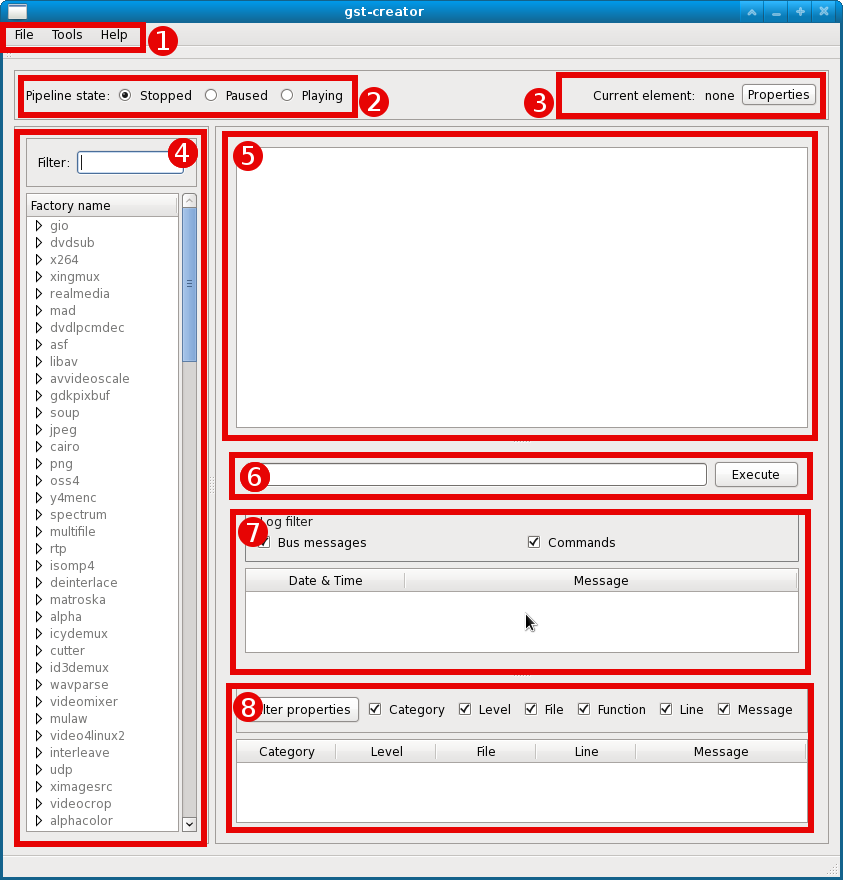
\includegraphics[width=160mm]{img/main-window.png}
  \caption{Zrzut ekranu głównego okna programu}
  \label{fig:mainWindow}
\end{figure}
\subsubsection{Inspektor obiektów}
\subsubsection{Wiersz poleceń}
Wiersz poleceń umożliwia budowę modelu na podstawie prostych komend interpretowanych przez program. Wiersz poleceń posiada również mechanizm podpowiadania składni (rysunek ~\ref{fig:commandLine}), który ma na celu przyśpieszenie i ułatwienie użytkownikowi pracy z programem. W przypadku słów kluczowych, wielkość liter nie ma znaczenia. Poniżej przedstawiona zostanie syntaktyka poszczególnych poleceń. 
\begin{figure}[H]
  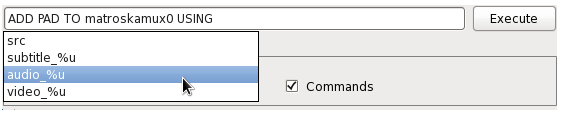
\includegraphics[width=140mm]{img/command-line.png}
  \caption{Mechanizm podpowiadania składni w wierszu poleceń}
  \label{fig:commandLine}
\end{figure}
\begin{itemize}
  \setlength{\itemsep}{0em}
\item \textbf{ADD} - dodaje element do modelu programu lub dodaje gniazdo do elementu.
\underline{Składnia:} \\
\texttt{ADD \\
\hspace*{2em} \{ELEMENT \textit{fabryka} [\textit{nazwa\_elementu}]\} | \\
\hspace*{2em} \{PAD TO \textit{element} USING \textit{szablon} [\textit{nazwa\_gniazda}]\} }
\begin{itemize}
\item \textit{fabryka} - nazwa fabryki, jaka ma zostać użyta do skonstruowania elementu.
\item \textit{nazwa\_elementu} - nazwa dla nowo utworzonego elementu (parametr opcjonalny).
\item \textit{element} - nazwa elementu, do którego dodane zostanie gniazdo.
\item \textit{szablon} - schemat, na podstawie którego zostanie utworzone gniazdo.
\item \textit{nazwa\_gniazda} - nazwa dla nowo utworzonego gniazda (parametr opcjonalny).
\end{itemize}
\underline{Przykłady:} \\
\texttt{ADD ELEMENT giosink} \\
\texttt{ADD ELEMENT fakesrc fake-generator} \\
\texttt{ADD PAD TO tee0 USING src\_\%u} \\
\texttt{ADD PAD to matroskamux0 USING subtitle\_\%u sub1}
\cleardoublepage
\item \textbf{REMOVE} - usuwa element z modelu programu lub usuwa gniazdo z elementu. \\
\underline{Składnia:} \\
\texttt{REMOVE \\
\hspace*{2em} \{ELEMENT \textit{nazwa\_elementu}\} | \\
\hspace*{2em} \{PAD \textit{nazwa\_elementu}:\textit{nazwa\_gniazda}\}}
\begin{itemize}
\item \textit{nazwa\_elementu} - nazwa elementu, który ma zostać usunięty.
\item \textit{nazwa\_gniazda} - nazwa gniazda, które ma zostać usunięte.
\end{itemize}
\underline{Przykłady:} \\
\texttt{REMOVE ELEMENT videotestsrc0}
\texttt{REMOVE PAD matroskamux0:sub1}
\item \textbf{PROPERTY} - umożliwia zmianę właściwości elementu.
\underline{Składnia:} \\
\texttt{PROPERTY \textit{element} [\textit{właściwość} \textit{wartość}]}
\begin{itemize}
\item \textit{element} - nazwa elementu, którego właściwość będzie zmieniana.
\item \textit{właściwość} - nazwa właściwości, jaka powinna zostać zmieniona (parametr opcjonalny).
\item \textit{wartość} - nowa wartość dla zadanej właściwości (parametr opcjonalny). 
\end{itemize}
\underline{Przykłady:} \\
\texttt{PROPERTY videotestsrc0} \\
\texttt{PROPERTY filesink0 location /home/m.kolny/output.mkv} \\
\underline{Uwagi:} \\
Użycie polecenia \textit{PROPERTY} w wariancie jednoargumentowym nie spowoduje de facto zmiany żadnego parametru. Wynikiem wykonania takiego polecenia będzie za to wyświetlenia okna z listą wszystkich dostępnych parametrów dla danego elementu(rysunek ~\ref{fig:allPropertiesWindow}), z możliwością zmiany tych parametrów.
\begin{figure}[H]
  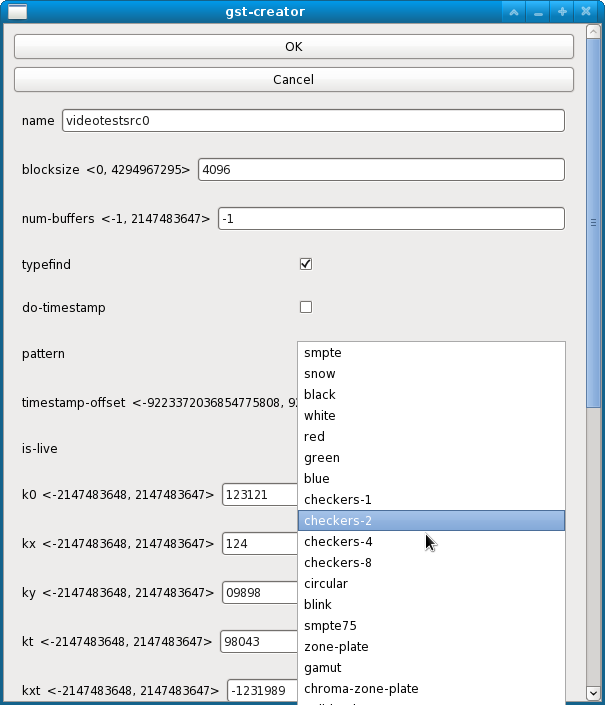
\includegraphics[width=150mm]{img/all-properties-window.png}
  \caption{Okno konfiguracji parametrów elementu \textit{videotestsrc0} - wynik wykonania polecenia \texttt{PROPERTY videoetstsrc0}}
  \label{fig:allPropertiesWindow}
\end{figure}
\cleardoublepage
\item \textbf{STATE} - zmienia stan modelu programu. \\
\underline{Składnia:} \\
\texttt{STATE STOP | PAUSE | PLAY} \\
\underline{Przykłady:} \\
\texttt{STATE STOP} \\
\texttt{STATE PLAY}
\item \textbf{CONNECT} - łączy ze sobą elementy lub gniazda. \\
\underline{Składnia:} \\
\texttt{CONNECT \\
\hspace*{2em} \{ELEMENT \textit{element\_źródłowy} WITH \textit{element\_docelowy}\} \\
\hspace*{2em} | \\
\hspace*{2em} \{PAD \textit{element\_źródłowy}:\textit{gniazdo\_źródłowe} WITH \\
\hspace*{4em} \textit{element\_docelowy}:\textit{gniazdo\_docelowe}\} \\
\hspace*{2em} [FUTURE]}
\begin{itemize}
\item \textit{element\_źródłowy} - nazwa elementu źródłowego dla połączenia.
\item \textit{element\_docelowy} - nazwa elementu docelowego dla połączenia.
\item \textit{gniazdo\_źródłowe} - nazwa gniazda w elementcie źródłowym.
\item \textit{gniazdo\_docelowe} - nazwa gniazda w elementcie docelowym.
\end{itemize}
\underline{Przykłady:} \\
\texttt{CONNECT ELEMENT matroskademux0 WITH avdec\_aac0 FUTURE} \\
\texttt{CONNECT ELEMENT videotestsrc0 WITH xvimagesink0} \\
\texttt{CONNECT pad matroskademux0:video\_\%u WITH xvimagesink0:sink FUTURE}
\texttt{CONNECT ELEMENT audiotestsrc0:src WITH autoaudiosink0:sink} \\
\underline{Uwagi:} \\
Słowo kluczowe \texttt{FUTURE} powinno zostać użyte w przypadku, gdy dane gniazdo nie istnieje na etapie projektowania modelu programu, a jego istnienie jest zależne od formatu wejściowych danych multimedialnych.
\cleardoublepage
\item \textbf{DISCONNECT} - rozłącza ze sobą elementy lub gniazda. \\
\underline{Składnia:} \\
\texttt{DISCONNECT \\
\hspace*{2em} \{ELEMENT \textit{element\_źródłowy} WITH \textit{element\_docelowy}\} \\
\hspace*{2em} | \\
\hspace*{2em} \{PAD \textit{element\_źródłowy}:\textit{gniazdo\_źródłowe} WITH \\
\hspace*{4em} \textit{element\_docelowy}:\textit{gniazdo\_docelowe}\}
}
\begin{itemize}
\item \textit{element\_źródłowy} - element źródłowy istniejącego połączenia.
\item \textit{element\_źródłowy} - element docelowy istniejącego połączenia.
\item \textit{gniazdo\_źródłowe} - gniazdo źródłowe istniejącego połączenia.
\item \textit{gniazdo\_docelowe} - gniazdo docelowe istniejącego połączenia.
\end{itemize}
\underline{Przykłady:} \\
\texttt{DISCONNECT ELEMENT queue0 WITH xvimagesink0} \\
\texttt{DISCONNECT PAD videotestsrc0 WITH autovideosink0}
\end{itemize}
\cleardoublepage
\section{Specyfikacja wewnętrzna}
\subsection{Rozwój biblioteki gstreamermm}
Biblioteka gstreamermm miała swój początek na początku 2008 roku. Wydanie dotyczyło wersji 0.9.1 biblioteki GStreamer, dla tego biblioteka-adapter otrzymała również taki numer. Biblioteka była rozwijana przez dwóch programistów: José Alburquerque oraz Murraya Cumminga. Jednak po wydaniu wersji 0.10.11, projekt nie był dalej rozwijany. Ponieważ w swojej codziennej pracy wykorzystuję bibliotekę GStreamer, postanowiłem dalej rozwijać projekt gstreamermm.
\subsubsection{Zmiany w blibliotece GStreamer}
Nowa wersja (1.0) biblioteki GStreamer wnosiła wiele zmian w stosunku do poprzedniej wersji biblioteki (0.10), adapter więc wymagał też wielu poprawek. 
\begin{itemize}
 \setlength{\itemsep}{0em}
  \item Wielu zmian dokonano w klasie \textit{GstBuffer}, która reprezentuje bufor danych w bibliotece GStreamer. Główna zmiana polegała na wprowadzeniu innego sposobu organizacji pamięci w buforze.
  \item Wiele funkcji związanych z gniazdami, zostało opartych o zapytania.
  \item Usunięte zostały wszystkie funkcje, oznaczone jako przestarzałe (ang. \textit{deprecated}).
\end{itemize}
Ponadto, w nowej wersji biblioteki GStreamer niektóre nazwy funkcji zostały zastąpione bardziej obrazowymi odpowiednikami. Zmieniała się również lista argumentów kilku funkcji.
Wszystkie powyższe zmiany musiały zostać uwzględnione w bibliotece adaptera.
\subsubsection{Wdrożenie nowego systemu testowania}
Do wersji 0.10, biblioteka gstreamermm nie była wyposażona w zautomatyzowany system testowania kodu. Tworzone były proste programy testujące, które należało uruchamiać ręcznie, a następnie śledzić wyniki wyświetlane na konsoli. Było to niewygodne, zwłaszcza dla dużej ilości testów. W wersji 1.0 biblioteki gstreamermm postanowiłem użyć popularnego systemu do testów automatycznych, \textbf{Google Test}. Po przeniesieniu testów na wspomniany wcześniej system, mogłem o wiele częściej uruchamiać wszystkie testy, i w łatwy sposób analizować rezultaty ich wykonania (rysunek ~\ref{fig:gtestScreen}). Użycie platformy testującej pozwoliło mi również na łatwiejsze pisanie testów.
\begin{figure}[H]
  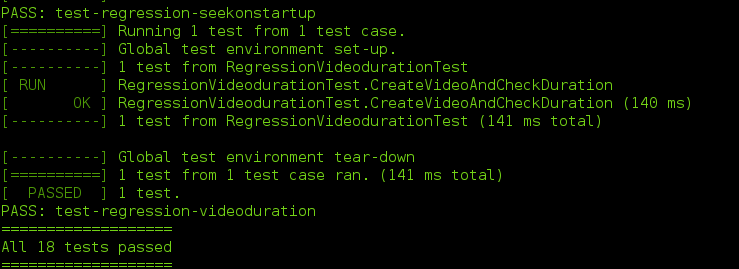
\includegraphics[width=150mm]{img/gtest-screen.png}
  \caption{Fragment zrzutu ekranu uruchomionego systemu Google Test dla projektu gstreamermm}
  \label{fig:gtestScreen}
\end{figure}
\subsubsection{Adaptacja modułu pisania wtyczek}
Biblioteka GStreamer opiera się o wtyczki, umożliwiające wprowadzenie do systemu dowolnego algorytmu. Adapter gstreamermm w wersji wcześniejszej, niż 1.0, nie posiadał oficjalnie wsparcia do pisania własnych wtyczek w języku C++. Powstała jednak nieoficjalna implementacja (\cite{pepergithub}), która oferowała programiście wsparcie dla pisania własnych wtyczek. Zaaplikowałem moduł do oficjalnego repozytorium. Dopisałem również brakującą klasę, która ułatwiała programiście dostęp do klasy danego elementu wtyczki.
\subsubsection{Poprawki w generatorach kodu}
Przy rozwijaniu projektu gstreamermm, wystąpiło kilka problemów, które należało rozwiązać po stronie generatora kodu. Jednym z nich był brak możliwości wprowadzenia wartości typu wyliczeniowego jako definicji wieloargumentowej. Na listingu ~\ref{badEnumForGenerator} pokazany został kod, który z punktu widzenia generatora kodu, był niepoprawny.
    \begin{lstlisting}[caption=Przykładowy fragment niepoprawnego z punktu widzenia generatora kodu źródłowego, label=badEnumForGenerator]
typedef enum {
  GST_QUERY_UNKNOWN      = GST_QUERY_MAKE_TYPE
(0, 0),
  GST_QUERY_POSITION     = GST_QUERY_MAKE_TYPE 
(10, FLAG(BOTH)),
  GST_QUERY_DURATION     = GST_QUERY_MAKE_TYPE 
(20, FLAG(BOTH)),
    \end{lstlisting}

Po wygenerowaniu kodu na podstawie powyższej definicji, oczekiwanym wynikiem jest fragment przedstawiony na listingu ~\ref{expectedGeneratedEnum}, natomiast generator tworzył kod, zaprezentowany na listingu ~\ref{outputGeneratedEnum}. Poprawienie błędu polegało na zmodyfikowaniu reguł dla wyrażeń regularnych generatora.

    \begin{lstlisting}[caption=Oczekiwany wynik działania generatora kodu, label=badEnumForGenerator]
(define-flags-extended QueryType
  (in-module "Gst")
  (c-name "GstQueryType")
  (values
    '("unknown" "GST_QUERY_UNKNOWN" 
"GST_QUERY_MAKE_TYPE (0,  0)")
    '("position" "GST_QUERY_POSITION" 
"GST_QUERY_MAKE_TYPE (10,  FLAG(BOTH))")
    '("duration" "GST_QUERY_DURATION" 
"GST_QUERY_MAKE_TYPE (20,  FLAG(BOTH))")
    \end{lstlisting}

    \begin{lstlisting}[caption=Błędnie wygenerowany kod przez generator, label=badEnumForGenerator]
(define-enum-extended QueryType
  (in-module "Gst")
  (c-name "GstQueryType")
  (values
    '("gst-query-unknown" "GST_QUERY_UNKNOWN" 
"GST_QUERY_MAKE_TYPE (0")
    '("0)" "0)" "(GST_QUERY_MAKE_TYPE (0) + 1")
    '("gst-query-position" "GST_QUERY_POSITION" 
"GST_QUERY_MAKE_TYPE (10")
    '("flag(both))" "FLAG(BOTH))" 
"(GST_QUERY_MAKE_TYPE (10) + 1")
    '("gst-query-duration" "GST_QUERY_DURATION" 
"GST_QUERY_MAKE_TYPE (20")
    '("flag(both))" "FLAG(BOTH))" 
"(GST_QUERY_MAKE_TYPE (20) + 1")
    \end{lstlisting}

\subsection{Opis modułów}
\cleardoublepage
\begin{thebibliography}{9}

\bibitem{gstmainpage}
  http://gstreamer.freedesktop.org [9.12.2013]
\bibitem{devgnomepage}
  https://developer.gnome.org [9.12.2013]
\bibitem{pepergithub}
  https://github.com/peper0/gstreamermm-plugins [10.12.2013]

\end{thebibliography}
\end{document}
